\documentclass[a4paper&11pt]{article}
\usepackage{caption}
\usepackage{subcaption}
\usepackage{float}
\usepackage[caption = false]{subfig}
\usepackage{graphicx}

\newcommand{\subf}[2]{%
  {\small\begin{tabular}[t]{@{}c@{}}
  #1\\#2
  \end{tabular}}%
}  


\begin{document}
\section*{ Vehicle Routing - 5 Cities}
\subsection*{With Capacity Constraint and No Time Constraint}


\begin{center}
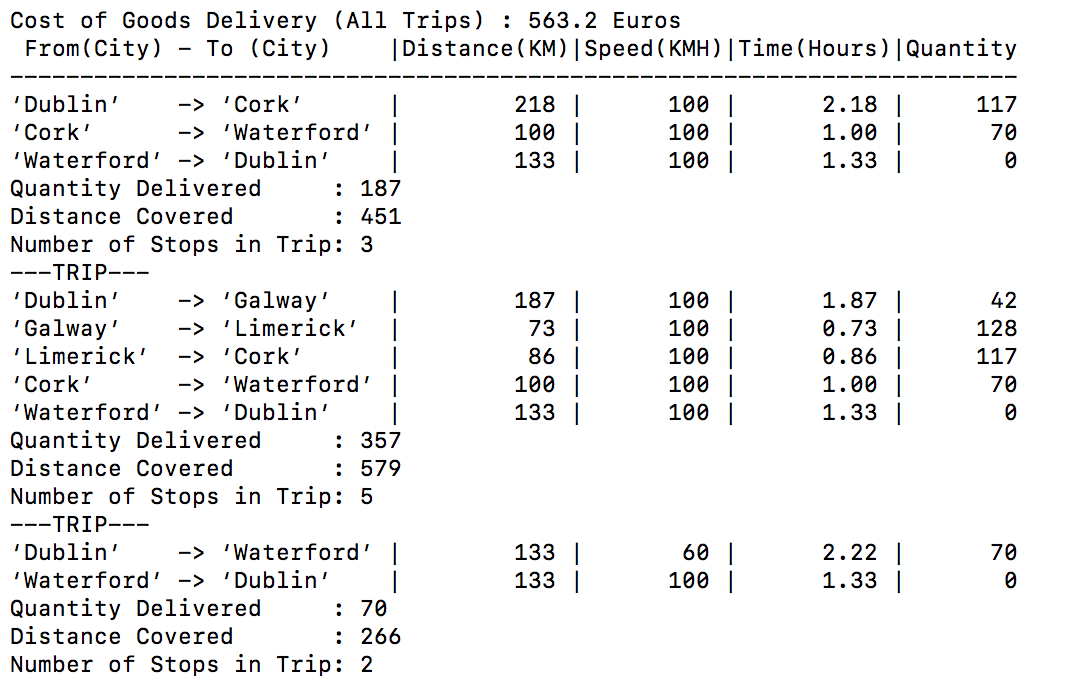
\includegraphics[scale=0.8]{fig1.png}
\begin{figure}[H]
\caption{Goods Delivery Optimal Cost :  With Capacity Constraint - Run1}
\end{figure}
\end{center}


\begin{center}
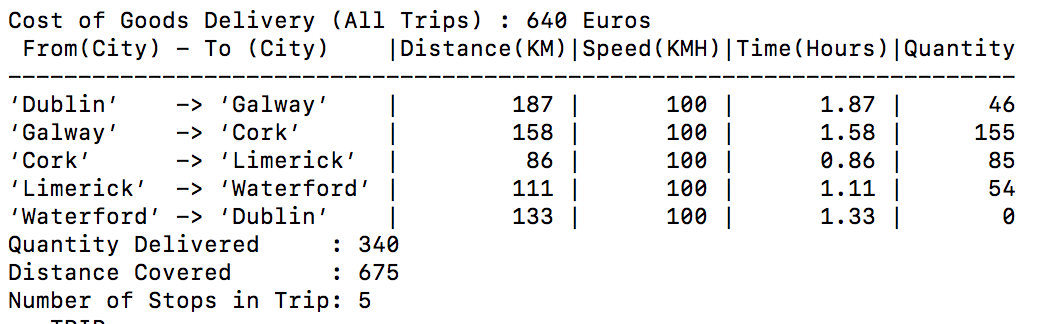
\includegraphics[scale=0.8]{fig2.png}
\begin{figure}[H]
\caption{Goods Delivery Optimal Cost :  With Capacity Constraint - Run2}
\end{figure}
\end{center}

\begin{center}
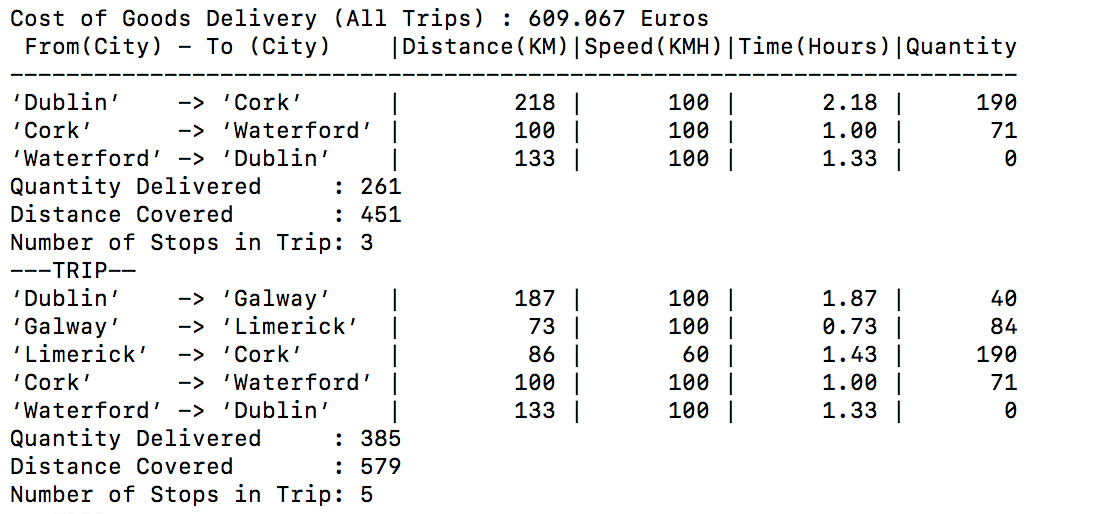
\includegraphics[scale=0.8]{fig3.png}
\begin{figure}[H]
\caption{Goods Delivery Optimal Cost :  With Capacity Constraint - Run3}
\end{figure}
\end{center}

\subsection*{With Capacity Constraint and Time Constraint}

\begin{center}
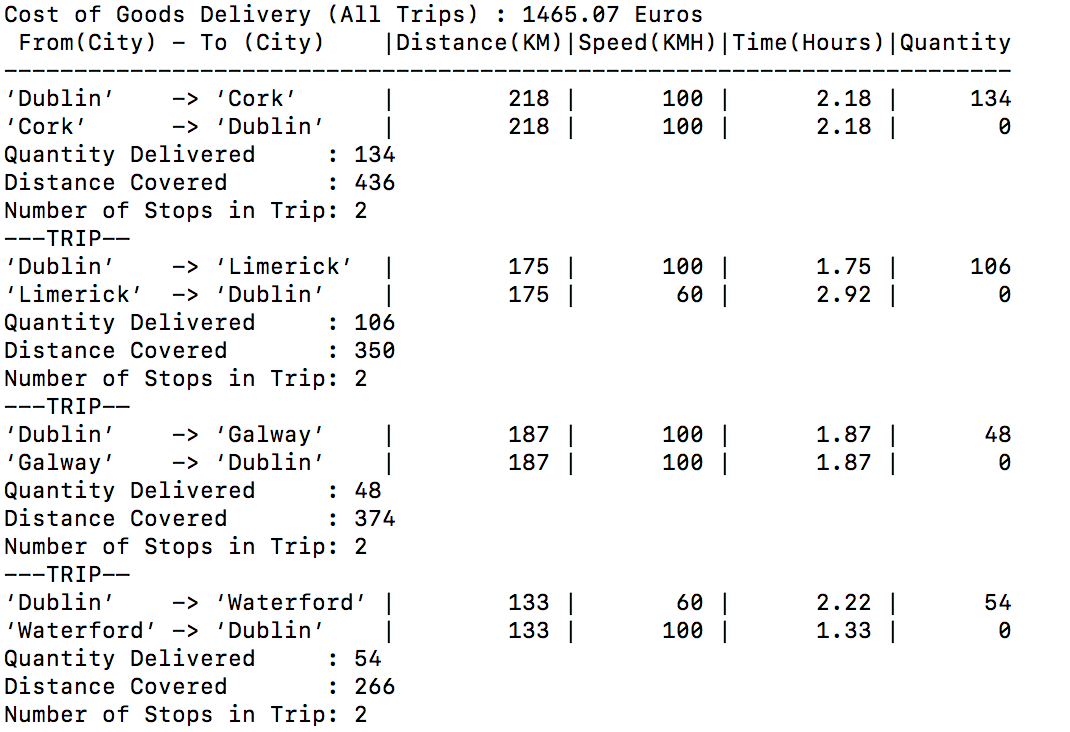
\includegraphics[scale=0.8]{fig4.png}
\begin{figure}[H]
\caption{Goods Delivery Optimal Cost :  With Capacity Constraint  and Time Constraint}
\end{figure}
\end{center}

\section*{Vehicle Routing  - 20 Cities}
\subsection*{With Capacity Constraint and No Time Constraint}

\begin{center}
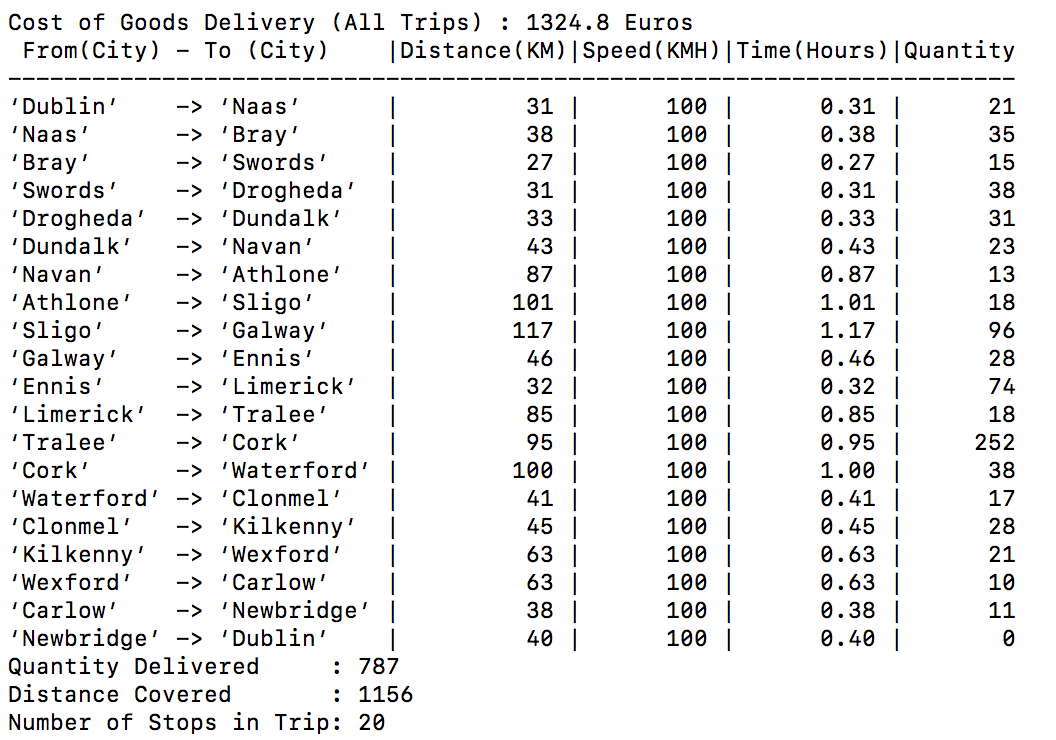
\includegraphics[scale=0.8]{20fig1.png}
\begin{figure}[H]
\caption{Goods Delivery Optimal Cost :  With Capacity Constraint - Run1}
\end{figure}
\end{center}


\begin{center}
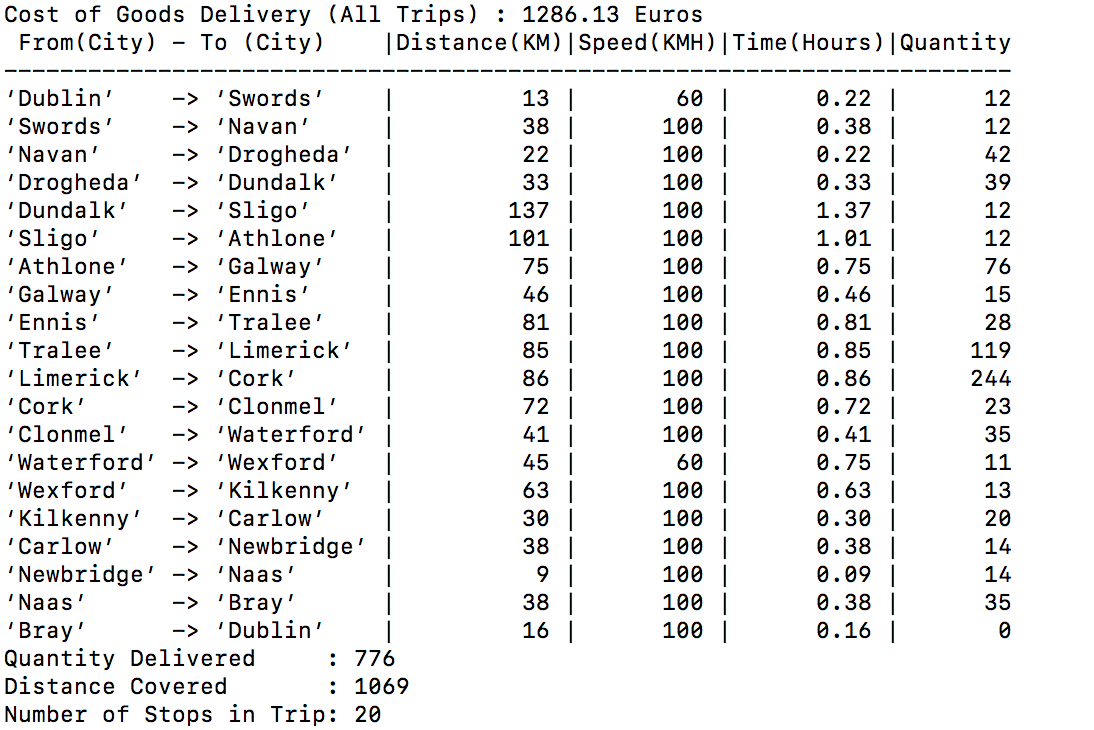
\includegraphics[scale=0.8]{20fig2.png}
\begin{figure}[H]
\caption{Goods Delivery Optimal Cost :  With Capacity Constraint - Run2}
\end{figure}
\end{center}

\begin{center}
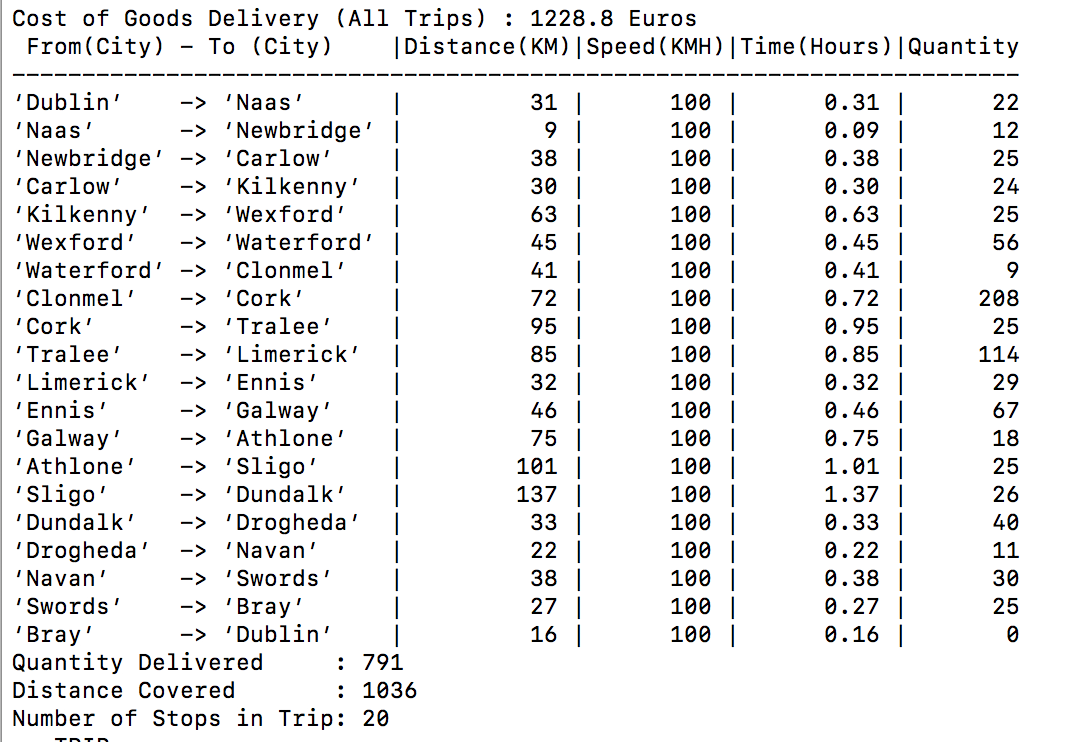
\includegraphics[scale=0.8]{20fig3.png}
\begin{figure}[H]
\caption{Goods Delivery Optimal Cost :  With Capacity Constraint - Run3}
\end{figure}
\end{center}

\subsection*{With Capacity Constraint and Time Constraint}

\begin{center}
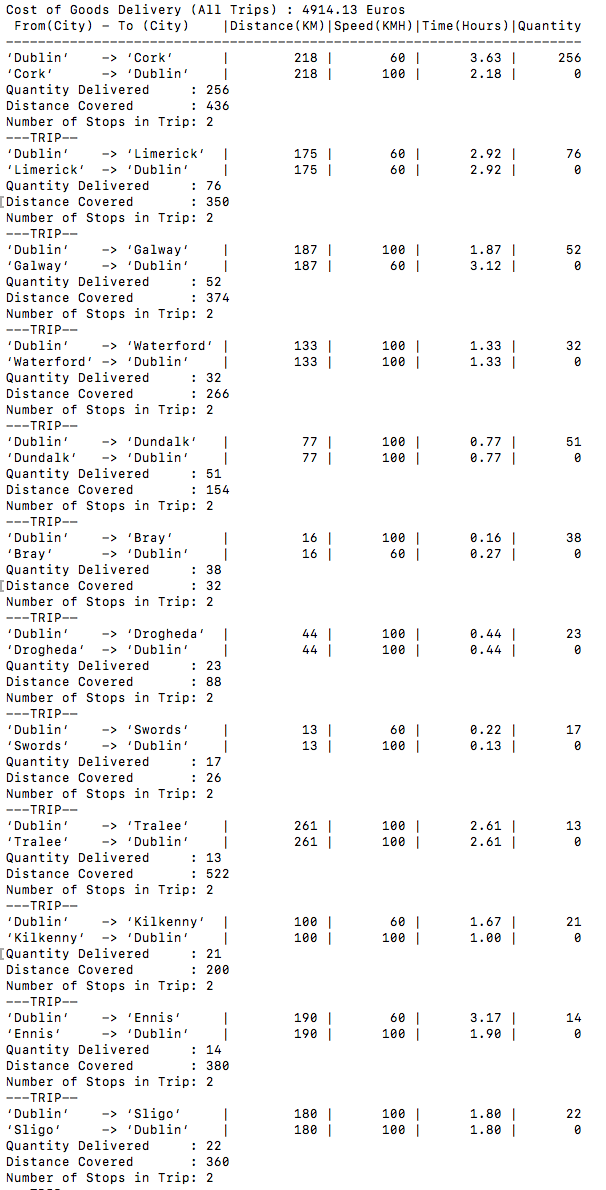
\includegraphics[scale=0.8]{20fig4.png}
\begin{figure}[H]
\caption{Goods Delivery Optimal Cost :  With Capacity Constraint  and Time Constraint}
\end{figure}
\end{center}

\section*{Vehicle Routing  - 30 Cities}
\subsection*{With Capacity Constraint and No Time Constraint}
\begin{center}
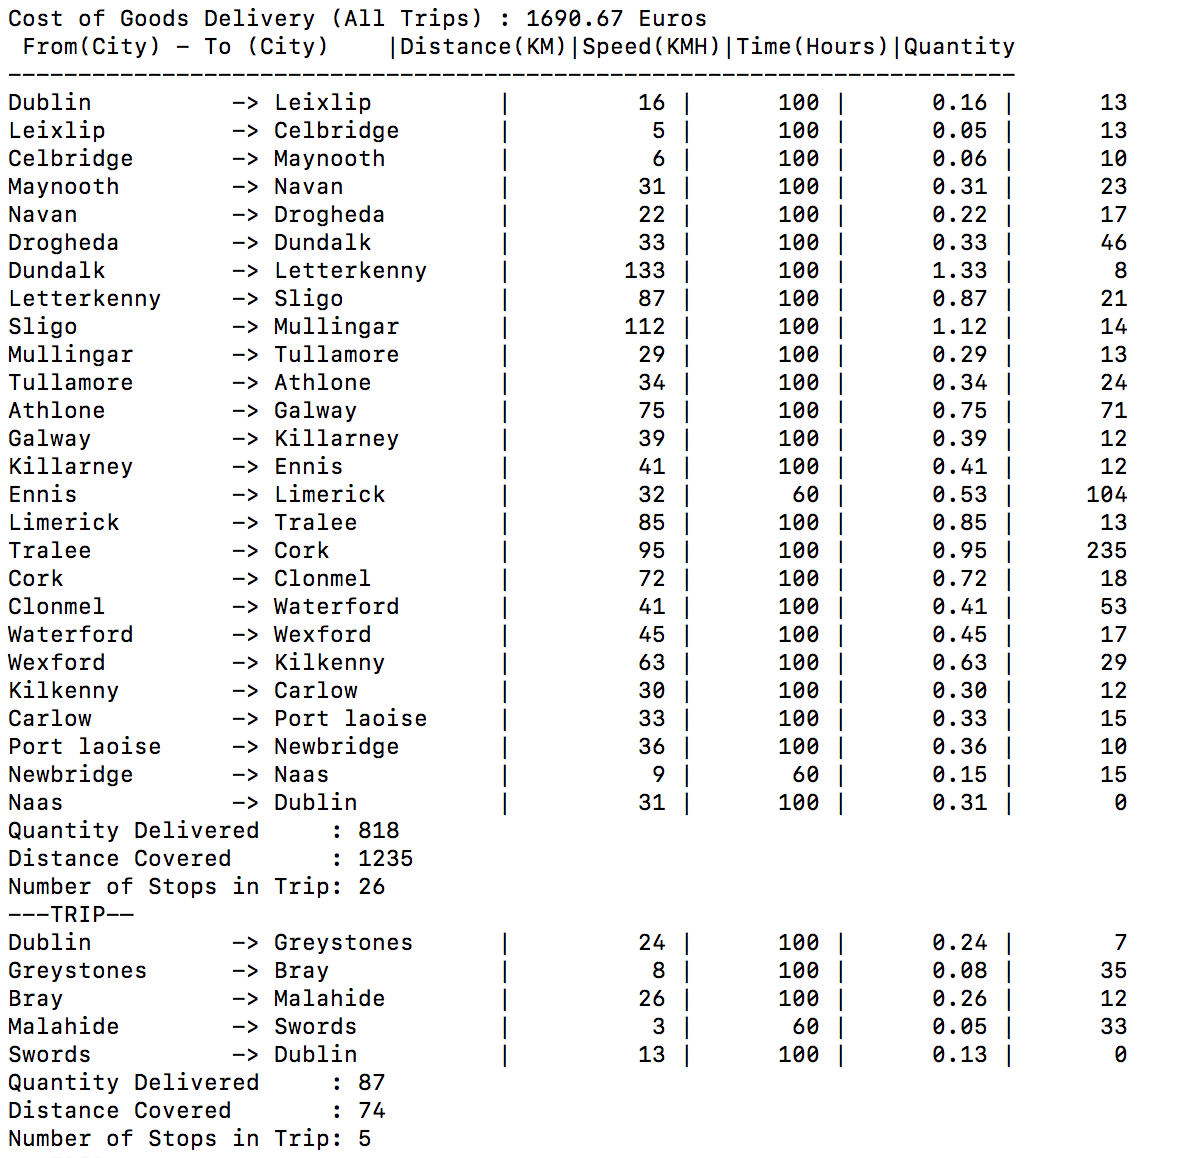
\includegraphics[scale=0.8]{30fig1.png}
\begin{figure}[H]
\caption{Goods Delivery Optimal Cost :  With Capacity Constraint - Run1}
\end{figure}
\end{center}


\begin{center}
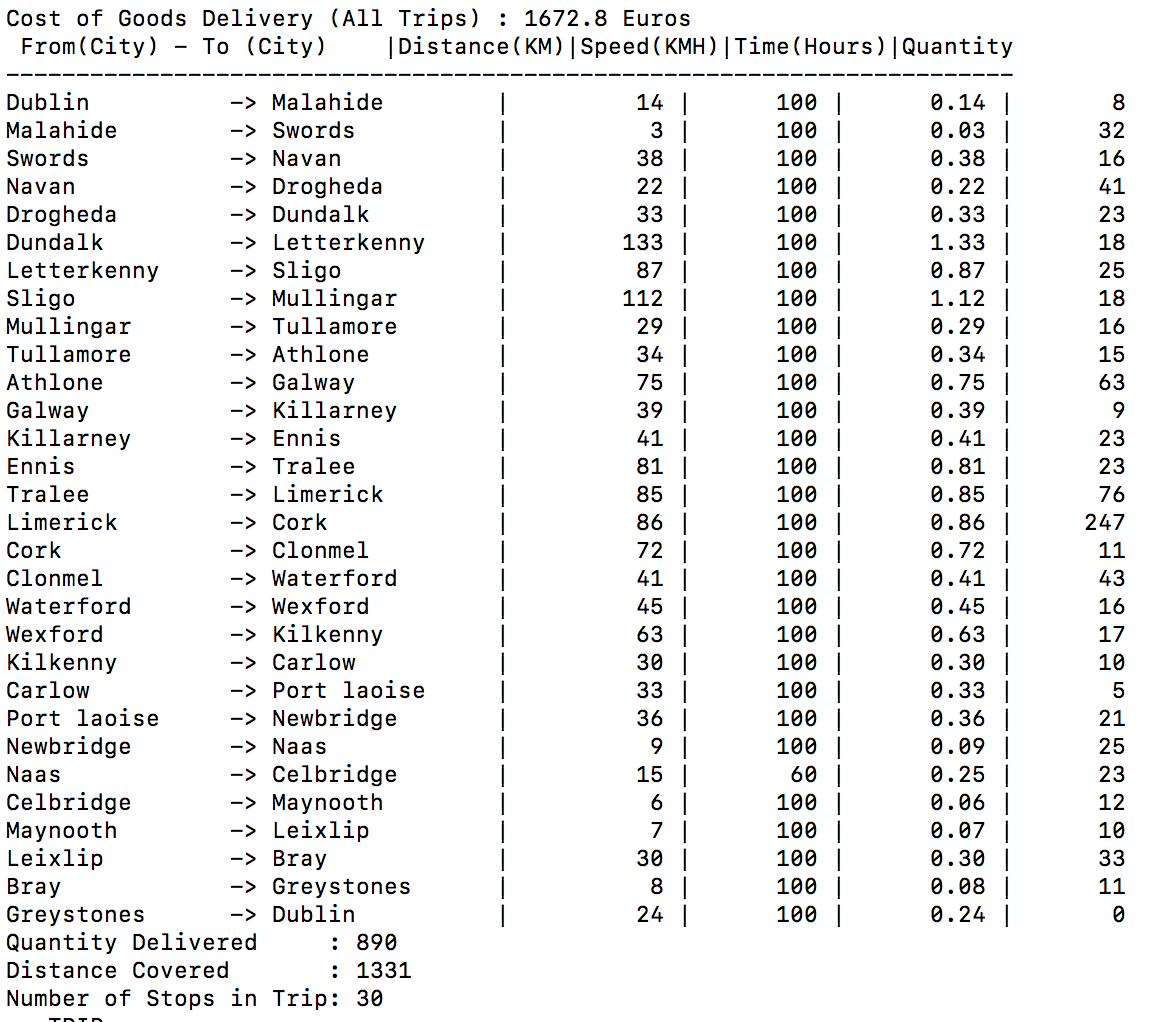
\includegraphics[scale=0.8]{30fig2.png}
\begin{figure}[H]
\caption{Goods Delivery Optimal Cost :  With Capacity Constraint - Run2}
\end{figure}
\end{center}

\begin{center}
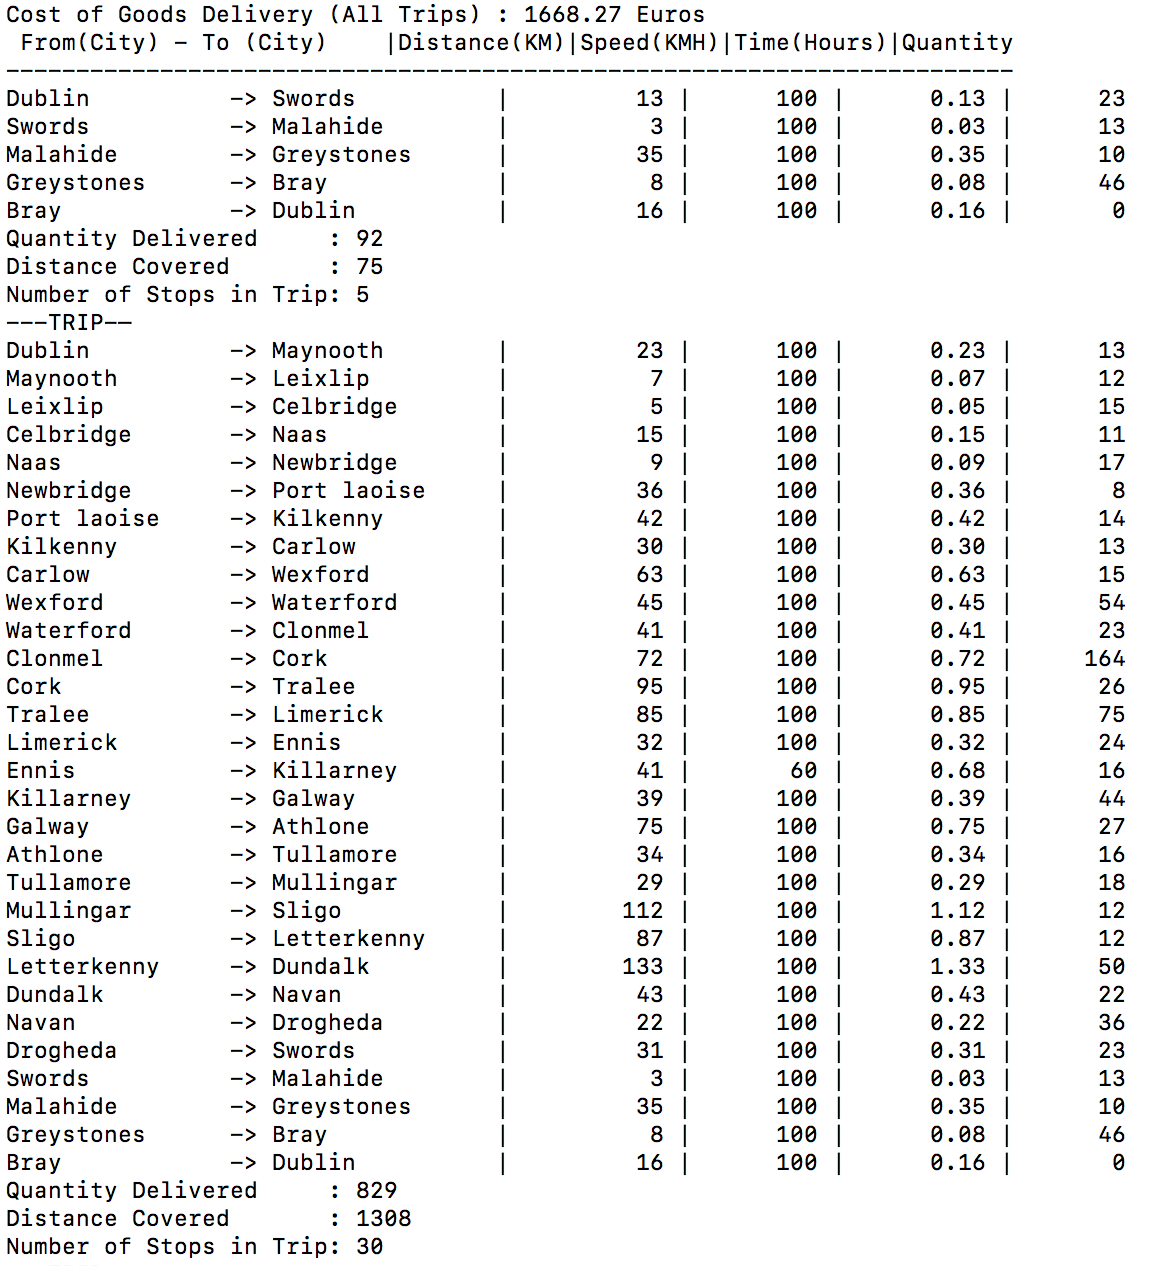
\includegraphics[scale=0.8]{30fig3.png}
\begin{figure}[H]
\caption{Goods Delivery Optimal Cost :  With Capacity Constraint - Run3}
\end{figure}
\end{center}

\subsection*{With Capacity Constraint and Time Constraint}

\begin{center}
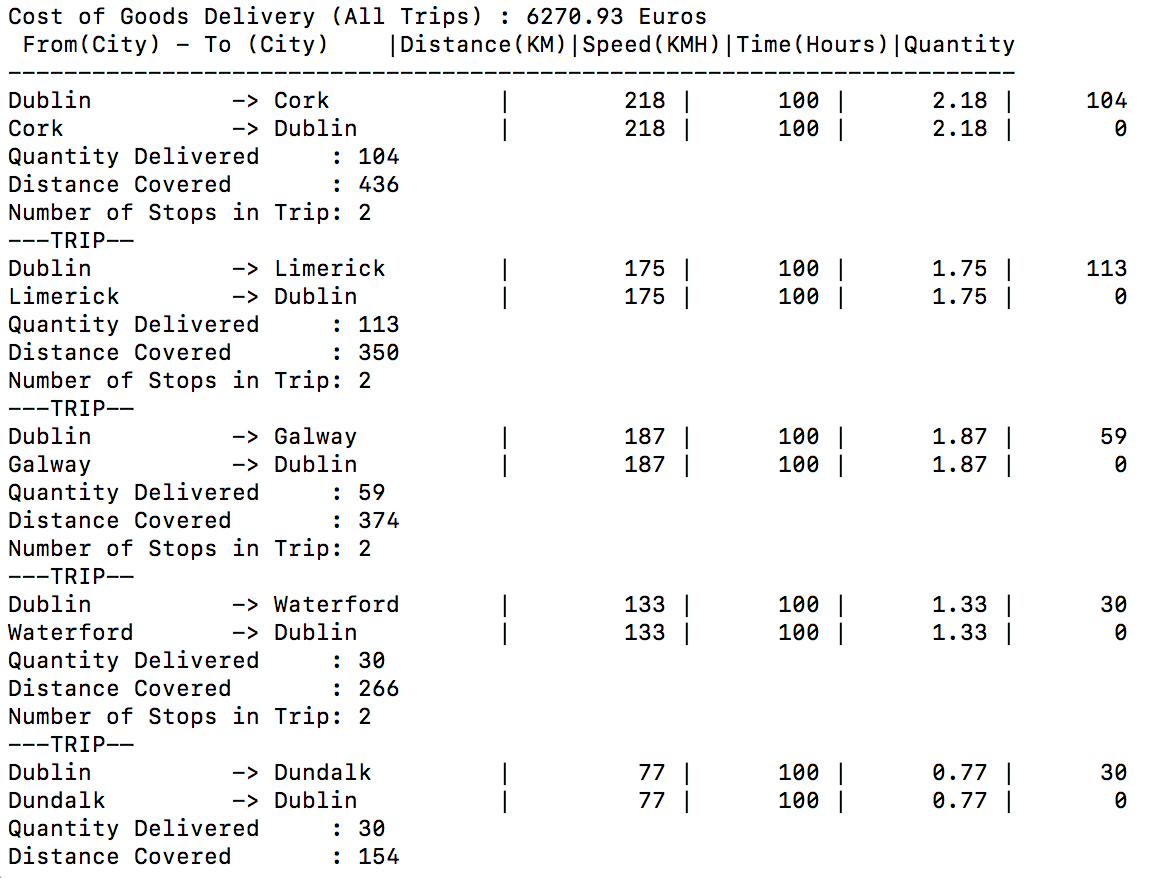
\includegraphics[scale=0.8]{30fig4.png}
\begin{figure}[H]
\caption{Goods Delivery Optimal Cost :  With Capacity Constraint  and Time Constraint}
\end{figure}
\end{center}



\end{document}